
\chapter{Geomechanical Modeling of Pecos}


\section{Dislocation (Fault Slip) Model}
\label{appen:okada}
\cite{Okada1992InternalDeformationDue} derived the analytical surface displacement field due to a finite rectangular fault slip in an elastic half-space. The Okada solutions provide three cases of displacement on a fault: strike-slip, dip-slip, tensile opening. In this study, we focused on the dip-slip case, because the Pecos area is in a normal faulting regime \cite{LundSnee2018}.  The assumption of predominant dip-slip along normal faults is also supported by fault plane solutions (TexNet Earthquake Catalog). 

Considering the case of dip slip on a finite rectangular fault (Figure \ref{fig:model-fault-geom}), the vertical surface displacement $u_z(x, y, 0)$ can be expressed as:
\begin{equation}
	u_{z}(x,y,0)=\frac{U_{2}}{2\pi }[u_{2}^{B}\sin \delta + u_{3}^{B}\cos \delta]
	\label{eq:okada}
\end{equation}
where $U_2$ is the magnitude of dip slip. The rest of terms on the right are determined by fault geometry parameters: the fault dip angle ($\delta$), the depth to the top of the fault ($Z$), the fault width along the dip direction ($W$), and the fault length along the strike direction ($L$). 

We located four faults based on InSAR observations, and assumed a uniform slip on each fault. We estimated the best-fit fault parameters for each fault independently by minimizing the objective function \cite{Du1992}:
\begin{equation}
	\arg \min_{U_{2,i}} \left \| \mathbf{G_i}U_{2,i}-\mathbf{d_i} \right \|^2_{2}  
	\label{eq:model-obj-1}
\end{equation}	  	
where $\mathbf{G_i}$ is the discrete Green’s function that maps a dip slip, $U_{2,i}$, on the $i^{th}$ rectangular fault to the observed vertical deformation at specific surface locations.  $\mathbf{G_i}$ is a function of fault geometry parameters as shown in Equation \eqref{eq:okada}. $\mathbf{d_i}$ is a vector of vertical deformation observations associated with the $i^{th}$ fault from InSAR data.

Through a grid-search, we solved for the fault dip angle, the depth to the top of the fault, the width along the dip direction, and the magnitude of dip slip on each fault to minimize the sum of squared residuals normalized by the data error of 1 cm (Normalized Sum of Squared Residuals; NSSR). The fault length in the strike direction is set to be sufficiently long to satisfy the plane strain condition. As an example, Figure \ref{fig:fault-supplement-nssr} shows how the data misfit varies with fault parameters for fault \#3. The maximum R-squared ($R^2$) values for the best-fit fault parameters are in the range of 0.95 and generally agree with the fault parameters that satisfy the minimum NSSR. 

The best-fit fault parameters of the four faults are listed in Table \ref{tab:geo-mech-fault}, which produce 3D surface deformation patterns as shown in Figure \ref{fig:fault-model-xyz}. To illustrate how surface deformation observations are related to the model parameters, Figure \ref{fig:fault-supplement2} shows the estimated surface subsidence associated with the fault \#3 long the B-B' transect with various fault properties. The ratio of the uplift volume to the subsidence volume is a function of the seismic potency and the fault dip angle \cite{Segall2019integrated}. Based on the results in Figure \ref{fig:fault-supplement2} (a), the fault dip angle dominantly controls the uplift volume relative to the subsidence volume. The slope from the uplift on the footwall to the subsidence on the hanging wall becomes steeper as the fault becomes shallower (Figure \ref{fig:fault-supplement2} (b)). The fault width, as measured along the the dip direction, mostly contributes to the width of the subsidence bowl (Figure \ref{fig:fault-supplement2} (c)).  The dip-slip magnitude only has impact on the amplitude of the curve without any influence on the shape of the surface deformation (Figure \ref{fig:fault-supplement2} (d)).




\begin{figure}
	\centering
	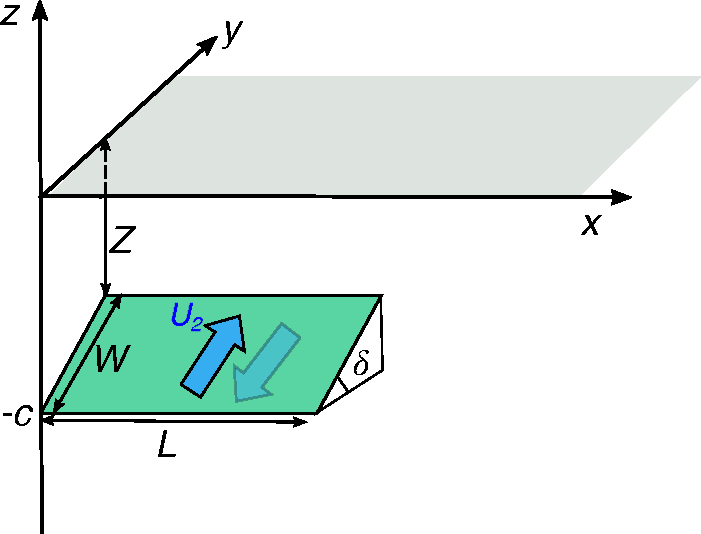
\includegraphics[width=\textwidth]{paper1-permian/figures/supplement/figureS6-fault-geom.pdf}
	\caption[A finite rectangular fault model from \cite{Okada1992InternalDeformationDue}]{A finite rectangular fault model from \cite{Okada1992InternalDeformationDue}. Here $U_2$ is the magnitude of dip slip (positive in reverse fault direction), $\delta$ is the dip angle, $Z$ is the depth to the top of the fault, $c$ is the depth to the bottom of the fault, $L$ is the length along the strike direction, and $W$ is the width along the dip direction.}
	\label{fig:model-fault-geom}
\end{figure}

\begin{table}
	\centering
	\caption{Best-fit fault parameters as derived from the dislocation model}
	\begin{tabular}{c|cccc}
		& Fault \#1      & Fault \#2      & Fault \#3      & Fault \#4      \\
		\hline
		1-Longitude ($^{\circ}$) & -103.563 & -103.589 & -103.585 & -103.529 \\
		1-Latitude ($^{\circ}$)  & 31.367   & 31.413   & 31.463   & 31.470   \\
		2-Longitude ($^{\circ}$) & -103.503 & -103.505 & -103.440 & -103.468 \\
		2-Latitude ($^{\circ}$)  & 31.337   & 31.355    & 31.374   & 31.432   \\
		Dip Angle ($^{\circ}$)   & 60       & 60       & 50       & 57.5       \\
		Depth (km)               & 0.91     & 0.91     & 1.07     & 1.52     \\
		Width (km)              & 0.61     & 0.30     & 1.07     & 0.61     \\
		Slip (cm)                & 9.1     & 15.2     & 9.1     & 15.2    \\
	\end{tabular}
	\label{tab:geo-mech-fault}
\end{table}

\begin{figure}
	\centering
	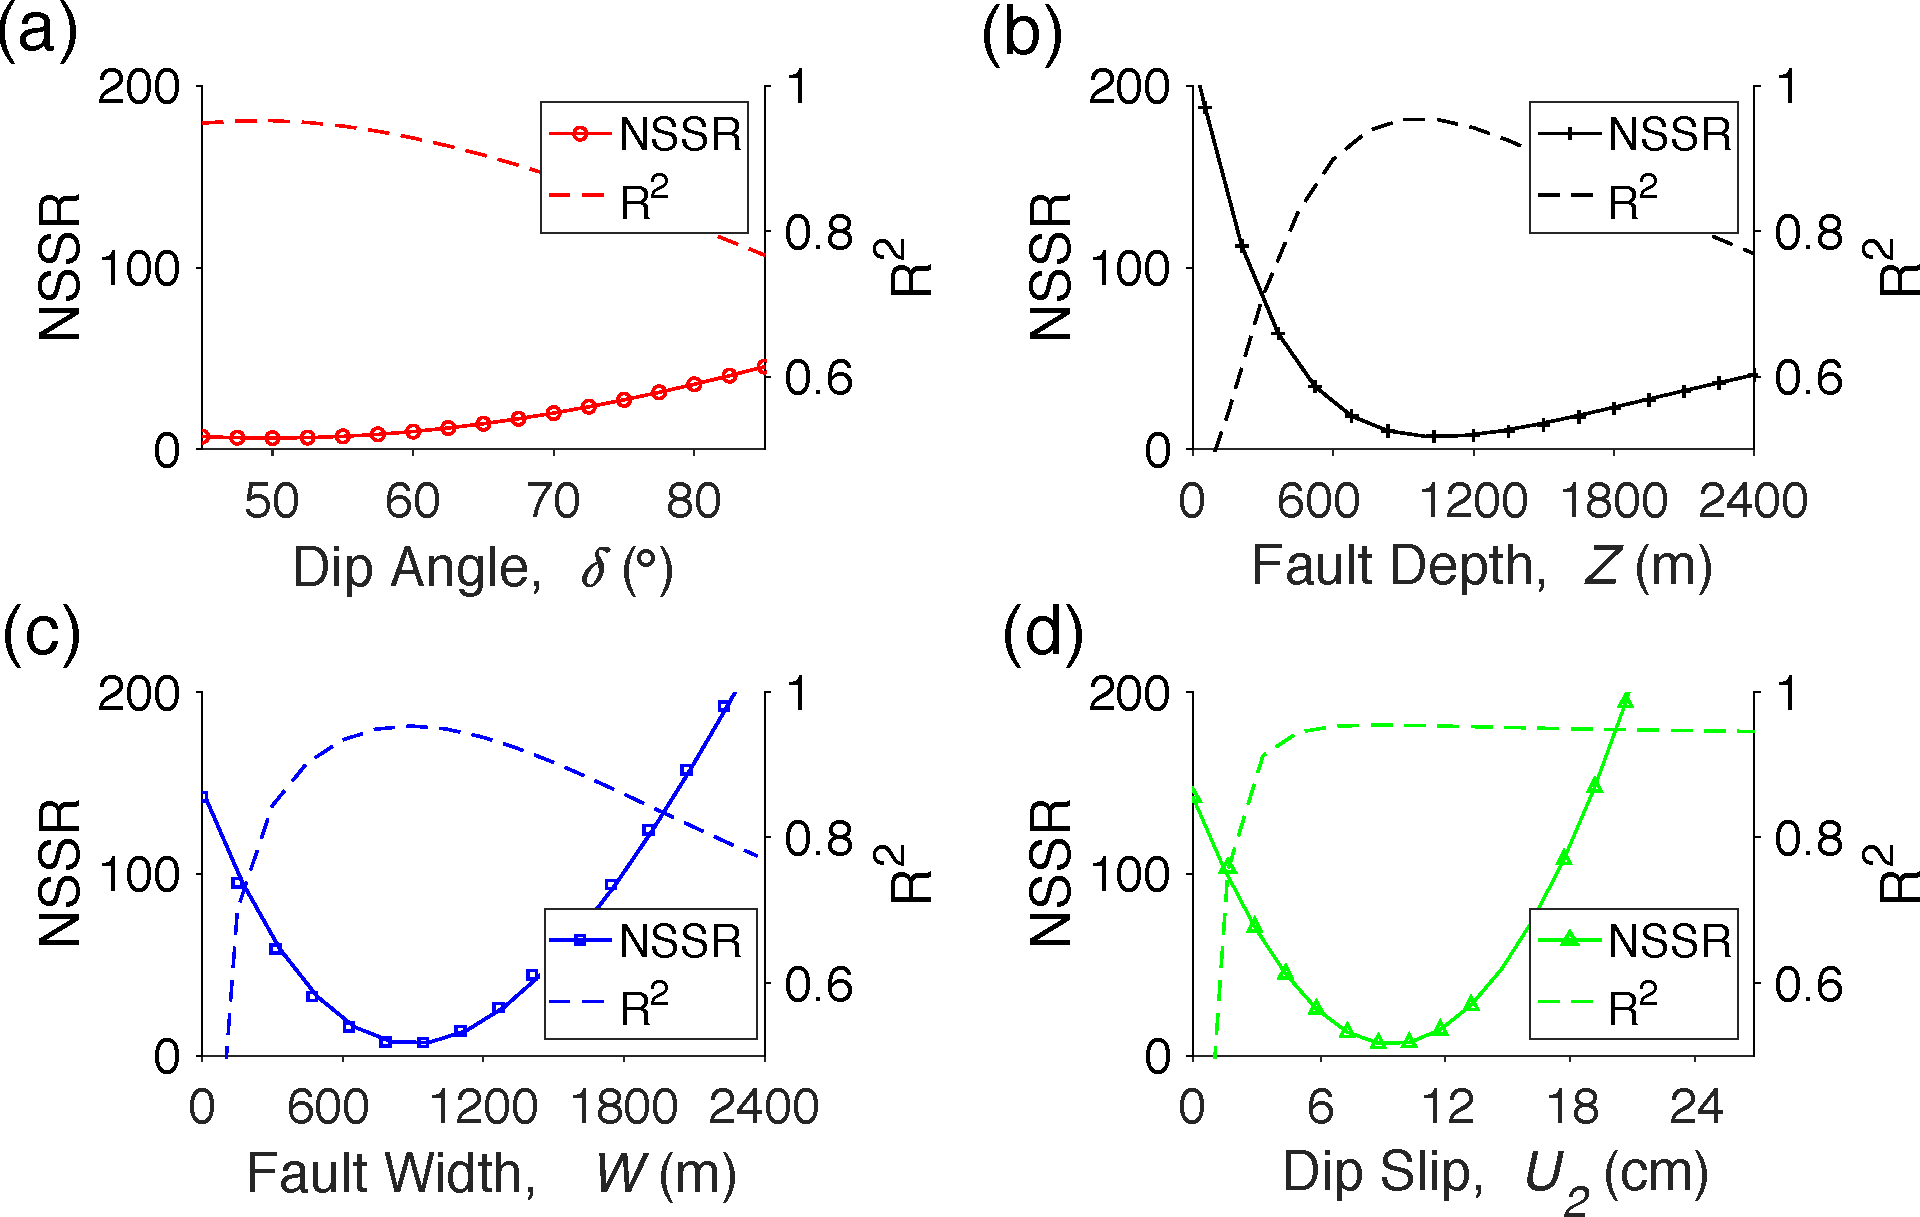
\includegraphics[width=.98\textwidth]{paper1-permian/figures/supplement/figureS7-fault-supplement-nssr.pdf}
	\caption[ Normalized Sum of Squared Residuals (NSSR) and R-squared for fault parameter inversion]{The Normalized Sum of Squared Residuals (NSSR) and R-squared ($ R^2 $) of fault \#3 relative to (a) fault dip angle ($ \delta $), (b) fault depth from the surface to the top of the fault ($ Z $), (c) fault width along the dip direction ($ W $), and (d) net dip slip magnitude ($ U_2 $).}
	\label{fig:fault-supplement-nssr}
\end{figure}

\begin{figure}
	\centering
	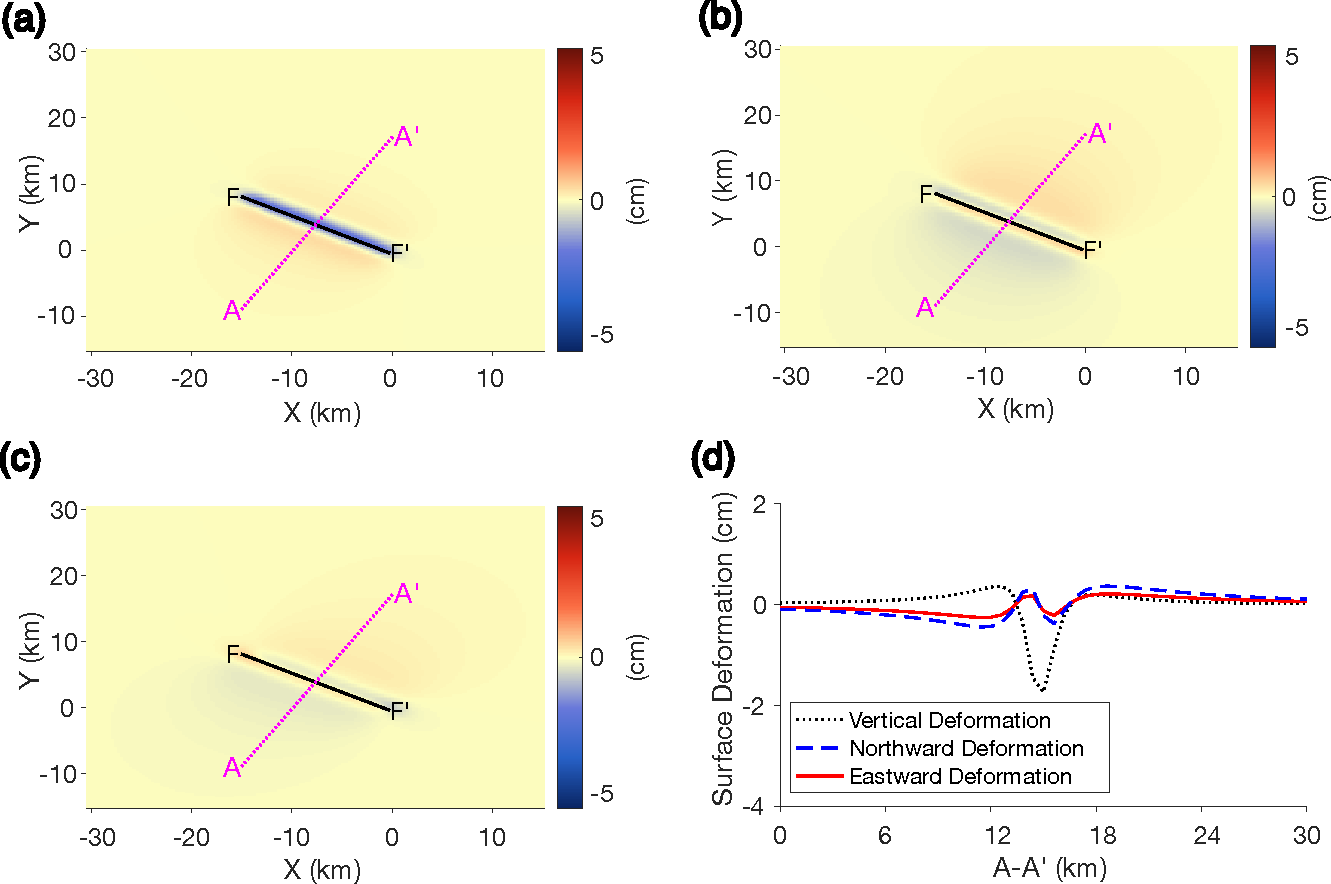
\includegraphics[width=\textwidth]{paper1-permian/figures/supplement/figureS8-fault-predicted-xyz.pdf}
	\caption[The predicted surface deformation from the Okada fault model]{The predicted surface deformation from the Okada fault model with best-fit parameters in the (a) vertical direction (positive means uplift), (b) northward direction (positive means north, negative means south), and (c) eastward direction (positive means east, negative means west). (d) Comparison of the 3D deformation profiles along A-A$^{'} $ transect that is perpendicular to fault plane.
	}
	\label{fig:fault-model-xyz}
\end{figure}

\begin{figure}
	\centering
	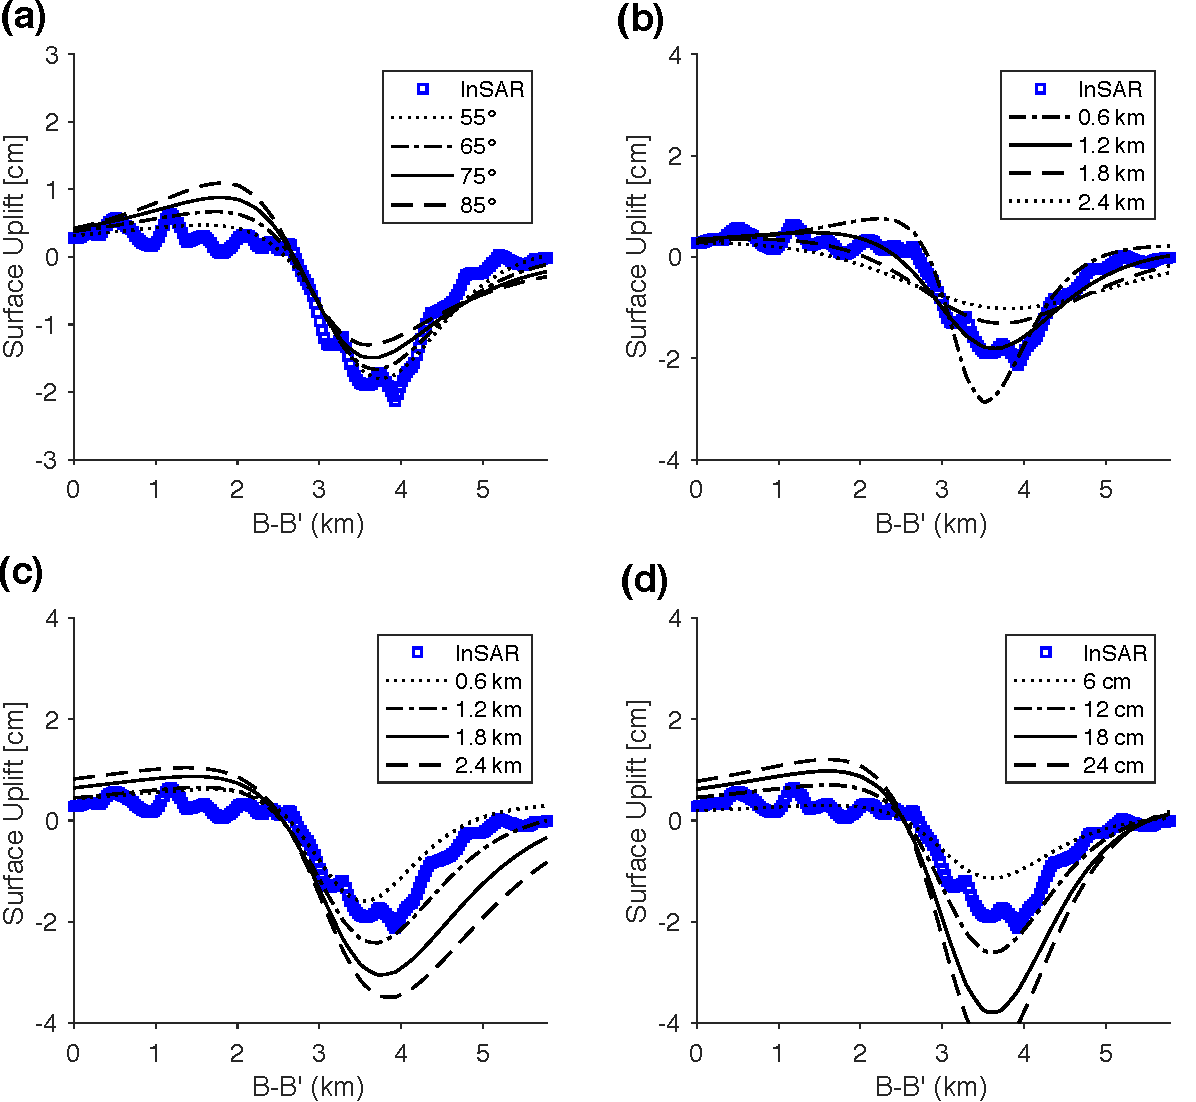
\includegraphics[width=\textwidth]{paper1-permian/figures/supplement/figureS9-fault-supplement2.pdf}
	\caption[Estimated surface subsidence along the B-B' transect associated]{Estimated surface subsidence along the B-B' transect associated with fault \#3 with various fault properties: (a) fault dip angle ($ \delta $) of 55$ ^{\circ} $, 65$ ^{\circ} $, 75$ ^{\circ} $, 85$ ^{\circ} $, (b) fault depth from the surface to the top of the fault ($ Z $) of 0.6 km, 1.2 km, 1.8 km, 2.4 km, (c) fault width along the dip direction, $ W $) of 0.6 km, 1.2 km, 1.8 km, 2.4 km, and (d) net dip slip magnitude ($ U_2 $) of 6 cm, 12 cm, 18 cm, 24 cm.}
	\label{fig:fault-supplement2}
\end{figure}


\pagebreak

\section{ Cylindrical Reservoir Compaction/Subsidence Model}
\label{appen:model-compact}
\cite{Geertsma1973LandSubsidenceCompacting} derived the surface displacement field due to a uniform pressure drop of a cylindrical reservoir at a depth $D$ (Figure \ref{fig:model-reservoir-geom}). Under the assumption that the reservoir radius $R$ is larger than the reservoir height $H$, the cylindrical reservoir deforms primarily in the vertical direction. The magnitude of the reservoir compaction $\Delta H$ due to a pressure drop $\Delta P$ can be written as:
\begin{equation}
	\Delta H = H c_m \Delta P
	\label{eq:rcompact}
\end{equation}
Here the  uniaxial compaction coefficient $c_m$ can be expressed as
\begin{align}
	c_{m} &= \alpha_{p}\frac{1+\nu}{1-\nu}\frac{c_{b}}{3} 
\end{align}
where $\alpha_p$ is Biot's coefficient, $c_b$ is the bulk compressibility, and $\nu$ is the Poisson's ratio. Surface vertical deformation $u_z$ due to the reservoir compaction $\Delta H$ can be expressed as:
\begin{align}
	u_{z}(r,0) &= 2(1-\nu)\Delta HA(\rho,\eta) 
	\label{eq:reservoirDef}
\end{align}
where $ A(\rho,\eta) = R\int_{0}^{\infty}e^{-D\alpha}J_{1}(\alpha R)J_{0}(\alpha r) \, d\alpha$, $\rho = r/R$, and $\eta =  D/R$. The maximum surface deformation at $r = 0$ can be written as:
\begin{equation}
	{u_{z}}^{max} = 2(1-\nu)\Delta H(1-\frac{\eta}{\sqrt{1+\eta^{2}}})
\end{equation}

The best-fit compaction in the cylindrical reservoirs were determined by minimizing the objective function \cite{Du2001}:
\begin{equation}
	\arg \min_{\mathbf{\Delta H}} =\left \| \mathbf{G_R}\mathbf{\Delta H}-\mathbf{d_r} \right \|^2+\beta ^2\left \| \mathbf{H_L}\mathbf{\Delta H}-\mathbf{d_0} \right \|^2  \label{eq:model-obj-2}
\end{equation}
where $ \mathbf{G_R} $ is the discrete Green’s function that maps the compaction of cylindrical reservoirs $\mathbf{\Delta H}$ in the subsurface to the observed vertical deformation at specific surface locations. $\mathbf{G_R}$ is a function of reservoir geometry parameters as shown in Equation \eqref{eq:reservoirDef}. $\mathbf{d_r}$ is a vector of vertical deformation observations associated with the reservoir compaction. In this study, $\mathbf{d_r}$ is the difference between the InSAR-observed total vertical deformation and modeled vertical fault slip deformation, $ \beta^2 $ is the penalty factor that weights the smoothness constraint, and $ \mathbf{H_L} $ is the finite difference approximation of the Laplacian operator. The reservoir compaction is constrained to be negative, and $\mathbf{d_0} $ is set to be zero. 

Based on the production well data near Pecos, we discretized two layers of reservoirs in the subsurface: Delaware Mountain Group (DMG) at depth 1.52 km and Wolfcamp at depth 3.05 km (Figure \ref{fig:model-reservoir-wells}). The shallow groundwater level reservoirs were not included in the reservoir model, because the water levels in the groundwater aquifers in the Pecos area were stable over the time period of interest \cite{deng2020surface}. The producing wells in the DMG were predominantly located to the east of Pecos, and we set 25 cylindrical reservoirs with the radius of 0.83 km. In the Wolfcamp formation, the wells were producing over the entire region. We discretized the layer covering the entire area with 100 cylindrical reservoirs with the radius of 0.83 km.  


\begin{figure}
	\centering
	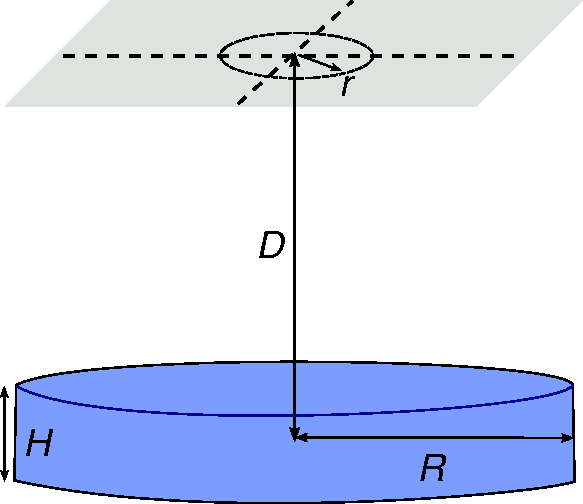
\includegraphics[width=.8\textwidth]{paper1-permian/figures/supplement/figureS10-reservoir-geom.pdf}
	\caption[Geometry of reservoir model in \cite{Geertsma1973LandSubsidenceCompacting}]{
		Geometry of reservoir model in \cite{Geertsma1973LandSubsidenceCompacting}, where $H$ is the reservoir height, $D$ is the reservoir depth, and $R$ is the reservoir radius.
	}
	\label{fig:model-reservoir-geom}
\end{figure}

\begin{figure}
	\centering
	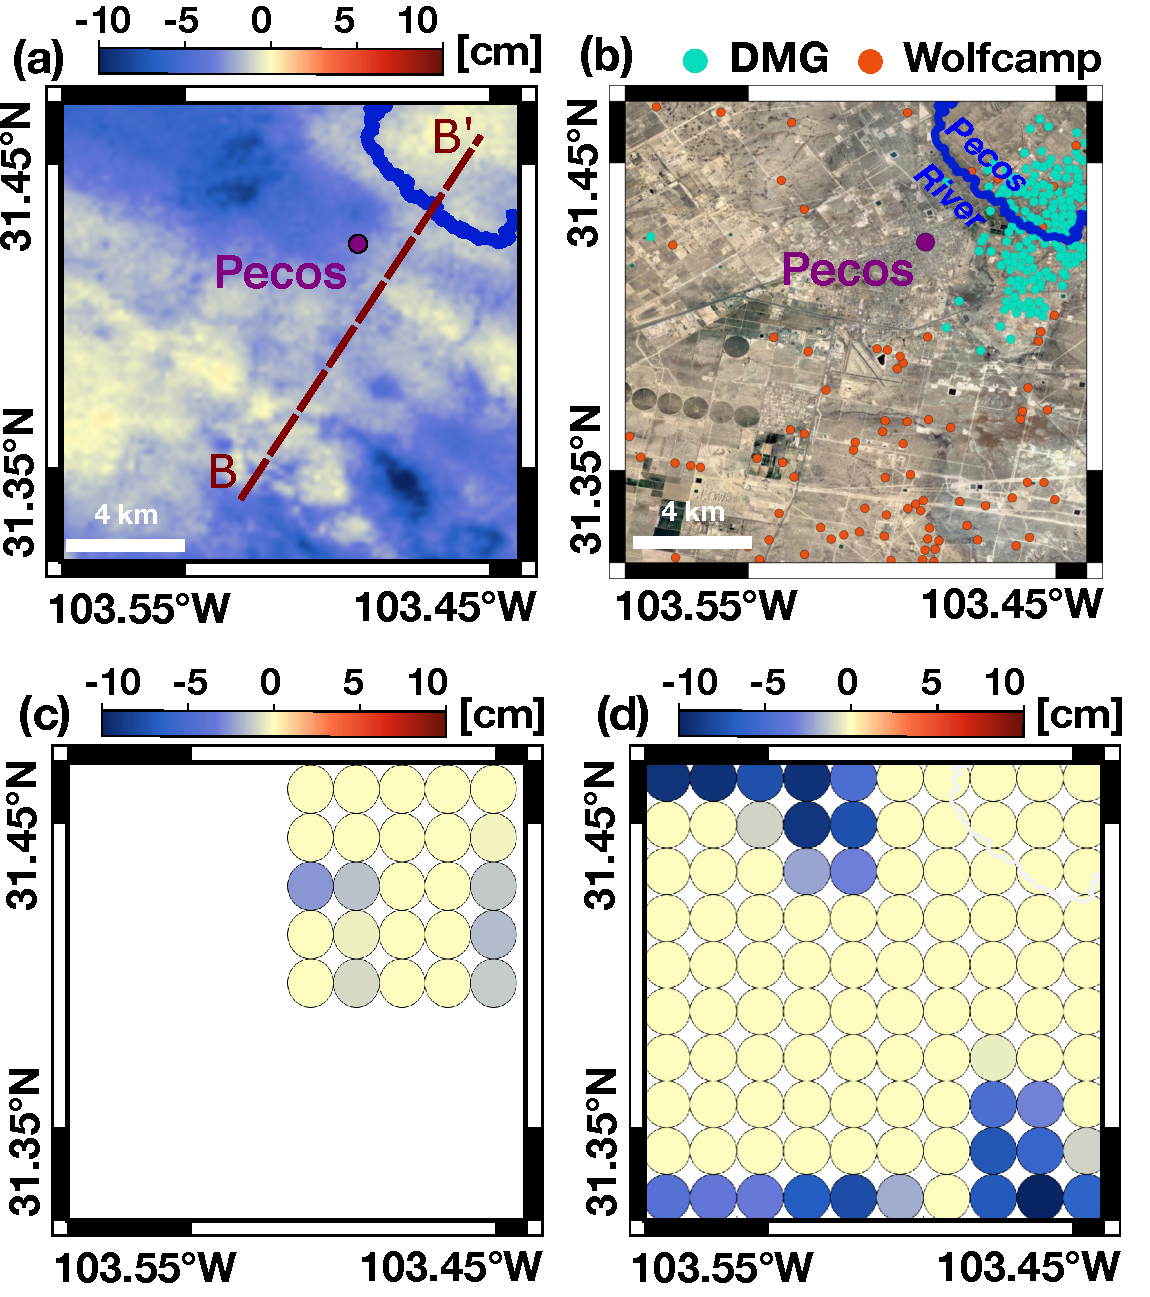
\includegraphics[width=.9\textwidth]{paper1-permian/figures/supplement/figureS11-reservoir-wells.pdf}
	\caption[Reservoir model setup for Delaware Mountain Group and Wolfcamp]{(a) Input for reservoir model: vertical surface deformation difference between InSAR and fault model (vertical surface deformation not explained by the fault model). (b) Producing well locations in near Pecos in the Delaware Mountain Group (DMG, cyan) and Wolfcamp (orange). Reservoir compaction values in (c) DMG reservoirs at depth 1.52km, and (d) Wolfcamp reservoirs at depth 3.05km. 
	}
	\label{fig:model-reservoir-wells}
\end{figure}



We utilized the pattern search optimization tool in MATLAB to minimize the objective function (Equation \eqref{eq:model-obj-2}). As the penalty factor $\beta^2$ decreases, the NSSR decreases, $ R^2 $ increases, and the modeled surface deformation better matches the InSAR data (Figure \ref{fig:model-reservoir-nssr}). Once the penalty factor ($ \beta^2 $) is smaller than 0.01, the NSSR and $ R^2 $ no longer change substantially. The best-fit reservoir compaction results ($ \beta^2 $ equals 0.01) for the two producing layers are shown in Figure \ref{fig:model-reservoir-wells}. While DMG reservoirs show some compaction (0 - 8 cm), the dominant compaction is in the Wolfcamp layer (0 - 27 cm). The production volume in DMG is as significant as in Wolfcamp. However, the dominant injection volume into DMG could maintain the reservoir pressure and minimize reservoir compaction. For certain regions in the Wolfcamp layer, the reservoir compaction appears to be discontinuous given the low $ \beta^2 $ value. We note that it is reasonable to observe localized compaction for tight shale formations, because the low formation permeability can cause heterogeneous pressure distribution during the depletion.

If appropriate mechanical properties of the formation are available, the distribution of reservoir pressure change and depleted zone can be evaluated by the reservoir compaction magnitudes based on Equation \eqref{eq:rcompact}. For example, if we assume Young’s modulus of 25 GPa, Poisson’s ratio of 0.25, and Biot’s coefficient of 0.67 based on published rock properties \cite{Shukla2013NanoindentationStudiesShales, Xu2015AnalysisStressVariations}, the localized maximum pressure drop is approximately 21 MPa. This is within a reasonable range given operational history in the area.



\begin{figure}
	\centering
	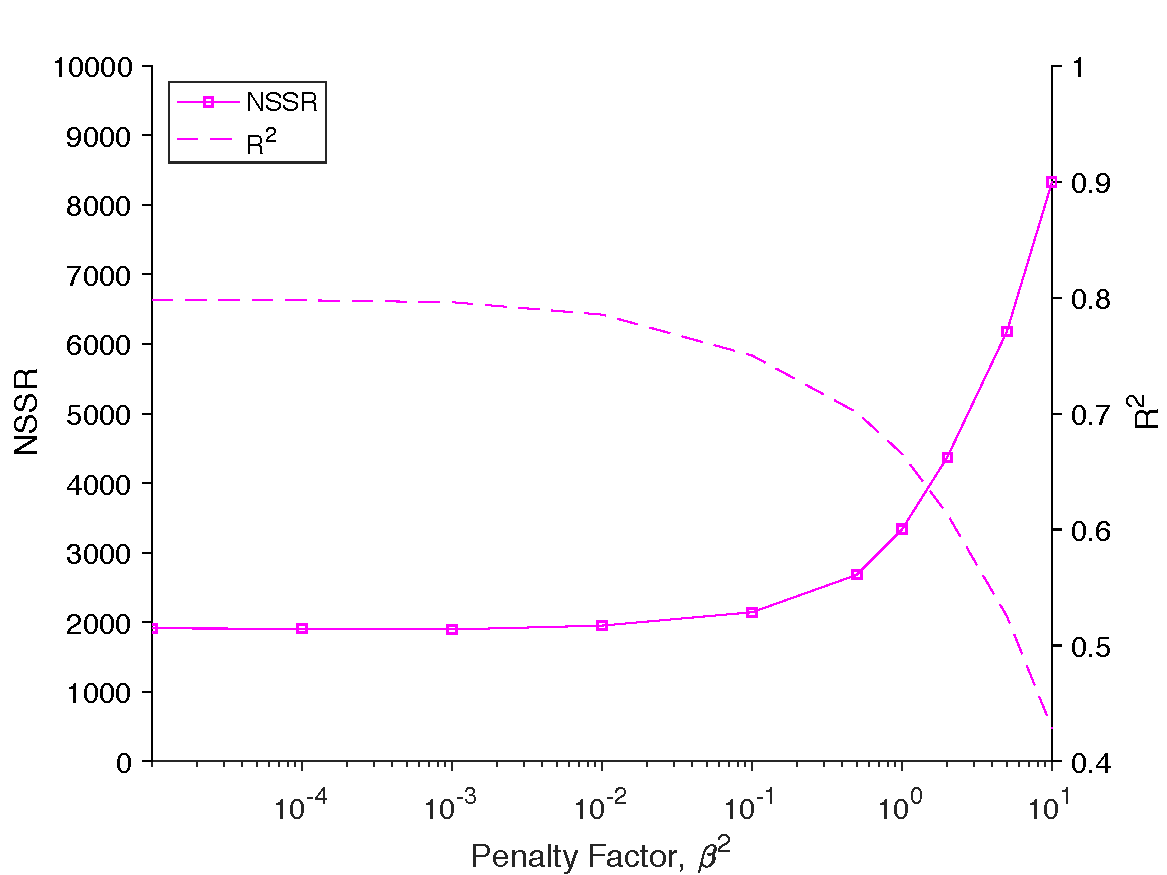
\includegraphics[width=\textwidth]{paper1-permian/figures/supplement/figureS12-reservoir-nssr.pdf}
	\caption[ Normalized Sum of Squared Residuals (NSSR) and R-squared for reservoir compaction model]{The Normalized Sum of Squared Residuals (NSSR) and R-squared ($ R^2 $) with varying penalty factor ($ \beta^2 $) for the discretized reservoir compaction model
	}
	\label{fig:model-reservoir-nssr}
\end{figure}

